\documentclass[article,final,14pt]{scrreprt}
\usepackage[utf8x]{inputenc}
\usepackage[russian]{babel}
\usepackage{amsfonts}
\usepackage{amsthm}
\usepackage{amssymb}
\usepackage{vmargin}
\usepackage{amsmath}
\usepackage{graphicx}
\usepackage{listings}
\usepackage{color}
\usepackage{multicol}
% \usepackage[Lenny]{fncychap}
\usepackage{xcolor}
\usepackage{hyperref}
\setpapersize{A4}
\setmarginsrb{2cm}{1.5cm}{1cm}{1.5cm}{0pt}{0mm}{0pt}{13mm}
\usepackage{indentfirst}
\sloppy
\DeclareGraphicsExtensions{.pdf,.png,.jpg}
\graphicspath{{images/}}

\definecolor{linkcolor}{HTML}{800000}
\definecolor{urlcolor}{HTML}{6495ED}

\hypersetup{pdfstartview=FitH,  linkcolor=linkcolor,urlcolor=urlcolor, colorlinks=true}

\setcounter{tocdepth}{2}
\linespread{1}
\begin{document}

\newtheorem{theorem}{Теорема}

\newtheorem{problem}{Задача}[chapter]

\newtheorem{lemma}{Лемма}[chapter]

\newtheorem{clair}{Утверждение}[chapter]

\newtheorem{definition}{Определение}[chapter]

\newtheorem{property}{Свойство}[chapter]

\newtheorem{conseq}{Следствие}[chapter]

\newtheorem{properties}{Свойства}[chapter]

\newtheorem*{remark}{Замечание}

\newenvironment{Proof}       
	{\par\noindent{\bf Доказательство.}}
	{\hfill$\blacksquare$}

\newenvironment{solution}       
	{\par\noindent{\bf Решение.}}
	{\hfill$\blacksquare$}

\newcommand{\red}[1]{\textbf{\color{red}#1}}
\newcommand{\blue}[1]{\textbf{\color{blue}#1}}

\def\ton#1{1,2,\dots,#1}
\def\Set#1#2{\left\{#1\colon#2\right\}}
\def\MYdef{\mathrel{\stackrel{\rm def}=}}

\begin{titlepage}
  \begin{center}
    \large
 
 	МОСКОВСКИЙ ГОСУДАРСТВЕННЫЙ УНИВЕРСИТЕТ ИМЕНИ М. В. ЛОМОНОСОВА

    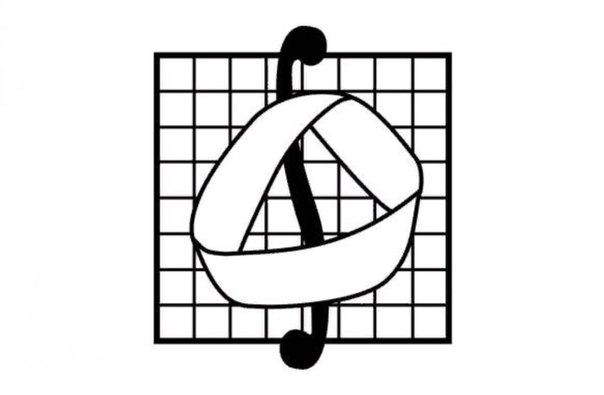
\includegraphics[scale=0.6]{mm.jpg} 
     
    Механико-математический факультет
    \vspace{0.25cm}

    Кафедра Вычислительной Математики
    \vspace{0.25cm}
 
    \textsc{Курсовая работа}\\[5mm]
     
    {\LARGE Восстановления отрезка по проекциям на плоскостях}
    \bigskip

    Конов Марк Андреевич
    \vspace{0.25cm}
     
    3 курс, группа 332
\end{center}
\vfill
 
\newlength{\ML}
\settowidth{\ML}{«\underline{\hspace{0.7cm}}» \underline{\hspace{2cm}}}
\hfill\begin{minipage}{0.5\textwidth}
  \begin{flushright}
     Научный руководитель\\
    к.ф.-м.н. \\
    Валединский Владимир Дмитриевич\\
    «\underline{\hspace{0.7cm}}» \underline{\hspace{2cm}} 2021 г.
  \end{flushright}
\end{minipage}%
\vfill
\bigskip
 
\begin{center}
  Москва, 2021 г.
\end{center}
\end{titlepage}
\newpage

\tableofcontents

\chapter{Описание задачи}

Даны несколько множеств (три) из $n$, $m$ и $p$ точек в пространстве. Необходимо найти отрезок, минимально удаленный от трех заданных множеств точек.

\begin{figure}[h]
	{ \noindent \centering
	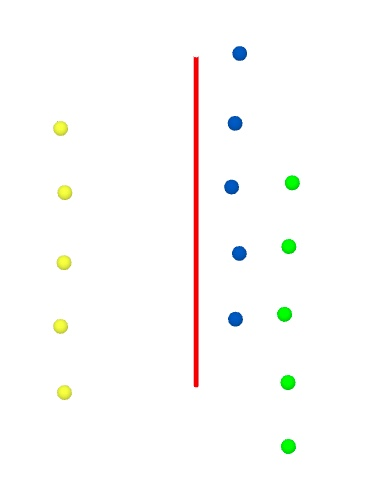
\includegraphics[scale=0.6]{1}
	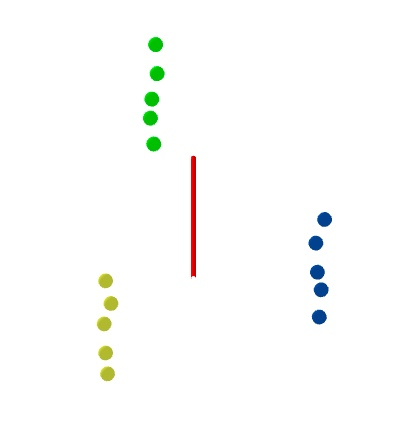
\includegraphics[scale=0.6]{2}
	\caption{Три множества и отрезок.}
	}
\end{figure}

\textbf{История задачи:}

Имеется отрезок и три плоскости. По трем заданным направлениям отрезок проецируется на на три плоскости, где мы получаем три отрезка.

Теперь стоит обратная задача. Пусть даны три множества точек, каждое из которых находится на соответствующей плоскости. Направления изначального проецирования заданы. По этим наборам точек на плоскостях и по направлениям процирования нужно найти исходный отрезок, который и проецировался на плоскости.

\newpage
\chapter{Алгоритм}

\section{Метод №1}\label{meth1}

Пусть имеем три множества точек: 

\begin{center}
	$P_1 = \Set{p_i^1 = (x_i^1, y_i^1, z_i^1)}{i=\ton n_1}$

	\vspace{0.3cm}
	$P_2 = \Set{p_i^2 = (x_i^2, y_i^2, z_i^2)}{i=\ton n_2}$

	\vspace{0.3cm}
	$P_3 = \Set{p_i^3 = (x_i^3, y_i^3, z_i^3)}{i=\ton n_3}$
\end{center}

Первым шагом необходимо построить прямые, приближающие данные три множества.

Пусть это следующие прямые: (можно найти, руководствуясь уже найденными алгоритмами)

\begin{center}
	$\mathit{l_1}: \; \begin{cases}
		x = x_0^1 + m^1 \cdot t \\
		y = y_0^1 + n^1 \cdot t \\
		z = z_0^1 + p^1 \cdot t
	\end{cases}$, где $t \in \mathbb{R}$ - параметр. 
\end{center}

\begin{center}
	$\mathit{l_2}: \; \begin{cases}
		x = x_0^2 + m^2 \cdot t \\
		y = y_0^2 + n^2 \cdot t \\
		z = z_0^2 + p^2 \cdot t
	\end{cases}$, где $t \in \mathbb{R}$ - параметр. 
\end{center}

\begin{center}
	$\mathit{l_3}: \; \begin{cases}
		x = x_0^3 + m^3 \cdot t \\
		y = y_0^3 + n^3 \cdot t \\
		z = z_0^3 + p^3 \cdot t
	\end{cases}$, где $t \in \mathbb{R}$ - параметр. 
\end{center}

Тогда мы имеем плоскости, перендикулярные нашим прямым:

\begin{center}
	$\mathit{\pi_1}: m^1 x + n^1 y + p^1 z + d = 0$

	\vspace{0.3cm}
	$\mathit{\pi_2}: m^2 x + n^2 y + p^2 z + d = 0$

	\vspace{0.3cm}
	$\mathit{\pi_3}: m^3 x + n^3 y + p^3 z + d = 0$

	\vspace{0.3cm}
	$d$ - любое число
\end{center}

Будем рассматривать усредненную плоскость $\mathit{\pi}: \; m x + n y + p z + d = 0$:

$$m = \frac{m^1+m^2+m^3}{3}, \; n = \frac{n^1+n^2+n^3}{3}, \; p = \frac{p^1+p^2+p^3}{3}$$

\begin{conseq}[\blue{построение объемлющей призмы}]\label{conseq1}
	Найдем две крайние точки: если плоскость $\pi$ проходит через эти точки, то все остальные точки находятся по одну сторону от плоскости. Практически это реализуется перебором точек, подбором коэффициента $d$ для того, чтобы плоскость проходила через данную точку, и подстановкой остальных точек в уравнение получившейся плоскости: если находим хотя бы пару точек с разными знаками при подстановке в уравнение плоскости, то работа с данной точкой заканчивается, и переходим к рассмотрению следующей.

	Благодаря описанной процедуре мы получаем две плоскости, являющиеся "крышками"  всех точек наших множеств. Таким образом, нами была фактически найдена призма, объемлющая все точки наших множеств: "крышки" являются основаниями призмы, а ребрами - наши прямые.
\end{conseq}

Будем брать каждую точку каждого множества и подбирать коэффициент $d$ так, чтобы плоскость проходила через текущую точку. Далее находятся две точки, являющиеся точками пересечения текущей плоскости и двух прямых, которые аппроксимируют два множества, которым текущая точка не принадлежит. Получаем треугольник в текущей плоскости, вершинами которого являются точки на прямых, аппроксимирующих исходные множества.

\vspace{0.3cm}
Найдем центр тяжести текущего треугольника, сохраним эту точку. После прохождения всех точек всех множеств мы получаем множество точек, являющихся центрами тяжести всех пройденных треугольников, параллельных плоскости $\pi$. Далее мы аапроксимируем данное множество прямой и рассматриваем ту ее часть, находящуюся между крайними точками полученного множества. Тем самым, искомый отрезок найден и задача решена.

\vspace{0.5cm}
\textbf{Алгоритм нахождения точки пересечения прямой и плоскости}

Пусть даны плоскость $\pi$ и прямая $\mathit{l}$:

$$\pi: \; ax+by+cz+d=0, \;\; \mathit{l}: \; 
\begin{cases}
	x = x_0 + m \cdot t \\
	y = y_0 + n \cdot t \\
	z = z_0 + p \cdot t
\end{cases}\text{, где }t \in \mathbb{R}\text{ - параметр.} $$

Найдем точку пересечения $\pi$ и $\mathit{l}$:

$$a (x_0 + m t) + b (y_0 + n t) + c (z_0 + p t) + d = 0 \; \Rightarrow \; $$

$$\; \Rightarrow \; t = - \frac{a x_0 + b y_0 + c z_0 + d}{a m + b n + c p}$$

\newpage
\section{Метод №2}\label{meth2}

Пусть имеем три множества точек: 

\begin{center}
	$P_1 = \Set{p_i^1 = (x_i^1, y_i^1, z_i^1)}{i=\ton n_1}$

	\vspace{0.3cm}
	$P_2 = \Set{p_i^2 = (x_i^2, y_i^2, z_i^2)}{i=\ton n_2}$

	\vspace{0.3cm}
	$P_3 = \Set{p_i^3 = (x_i^3, y_i^3, z_i^3)}{i=\ton n_3}$
\end{center}

Будем искать прямую $\mathit{l}$ такую, что сумма квадратов расстояний от нее до всех точек всех множеств, минимальна.

Будем искать прямую $\mathit{l}$ в параметрическом виде:

\begin{center}
	$\mathit{l}: \; \begin{cases}
		x = x_0 + m \cdot t \\
		y = y_0 + n \cdot t \\
		z = z_0 + p \cdot t
	\end{cases}$, где $t \in \mathbb{R}$ - параметр. 
\end{center}

Точку $M_0 = (x_0, y_0, z_0)$ найдем как центр тяжести всех точек всех множеств:

$$\begin{cases}
	x_0 = \frac{1}{n_1+n_2+n_3}\underset{i=1, j=1,2,3}{\overset{n_1+n_2+n_3}{\sum}}x_i^j \\
	y_0 = \frac{1}{n_1+n_2+n_3}\underset{i=1, j=1,2,3}{\overset{n_1+n_2+n_3}{\sum}}y_i^j \\
	z_0 = \frac{1}{n_1+n_2+n_3}\underset{i=1, j=1,2,3}{\overset{n_1+n_2+n_3}{\sum}}z_i^j
\end{cases}$$

По определению расстояние от точки $M_1$ до прямой $\mathit{l}$ определяется по следующей формуле:

$M_0 (x_0, y_0, z_0)$ - точка на прямой $\mathit{l}$

$\mathit{l} = (m, n, p)$ - напрявляющий вектор прямой

\begin{center}
	$d (M_1, \mathit{l}) = \frac{|[\overline{\mathit{l}}, \overline{M_0 M_1}]|}{|\overline{\mathit{l}}|}$
\end{center}

\begin{center}
	\begin{figure}[h]
	{ 	
		\noindent 
		\centering
		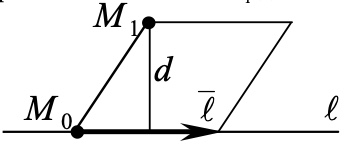
\includegraphics[scale=0.8]{3}
		\caption{Расстояние от точки до прямой.}
	}
\end{figure}
\end{center}

Распишем составляющие элементы формулы для расстояния:

$$|\overline{l}| = \sqrt{m^2 + n^2 + p^2}$$

$$\overline{M_0 M_1} = (x_1 - x_0, y_1 - y_0, z_1 - z_0)$$

$$[\overline{\mathit{l}}, \overline{M_0 M_1}] = \begin{vmatrix}
	\mathbf{i} & \mathbf{j} & \mathbf{k} \\
	m & n & p \\
	x_1 - x_0 & y_1 - y_0 & z_1 - z_0
\end{vmatrix} = $$

$$=\left(\begin{vmatrix}
	n & p \\
	y_1 - y_0 & z_1 - z_0
\end{vmatrix}, -\begin{vmatrix}
	m & p \\
	x_1 - x_0 & z_1 - z_0
\end{vmatrix}, \begin{vmatrix}
	m & n \\
	x_1 - x_0 & y_1 - y_0
\end{vmatrix}\right) = $$

$$= (n (z_1 - z_0) - p (y_1 - y_0), p (x_1 - x_0) - m (z_1 - z_0), m (y_1 - y_0) - n (x_1 - x_0)) = $$

$$ = (n \triangle_{z_1} - p \triangle_{y_1}, p \triangle_{x_1} - m \triangle_{z_1}, m \triangle_{y_1} - n \triangle_{x_1})\text{, где }\begin{cases}
	\triangle_{x_1} = x_1 - x_0 \\
	\triangle_{y_1} = y_1 - y_0 \\
	\triangle_{z_1} = z_1 - z_0
\end{cases}$$

$$|[\overline{\mathit{l}}, \overline{M_0 M_1}]| = \sqrt{(n \triangle_{z_1} - p \triangle_{y_1})^2 + (p \triangle_{x_1} - m \triangle_{z_1})^2 + (m \triangle_{y_1} - n \triangle_{x_1})^2}$$

Тогда формула расстояния принимает вид:

$$d (M_1, \mathit{l}) = \sqrt{\frac{(n \triangle_{z_1} - p \triangle_{y_1})^2 + (p \triangle_{x_1} - m \triangle_{z_1})^2 + (m \triangle_{y_1} - n \triangle_{x_1})^2}{m^2 + n^2 + p^2}}$$

Тогда наша мера примет вид:

$$\Lambda (\mathit{l}, P) = \sqrt{\underset{i=1}{\overset{n}{\sum}} \frac{(n \triangle_{z_i} - p \triangle_{y_i})^2 + (p \triangle_{x_i} - m \triangle_{z_i})^2 + (m \triangle_{y_i} - n \triangle_{x_i})^2}{m^2 + n^2 + p^2} } = $$

$$ = \frac{1}{\sqrt{m^2 + n^2 + p^2}} \sqrt{\underset{i=1}{\overset{n}{\sum}} \left( (n \triangle_{z_i} - p \triangle_{y_i})^2 + (p \triangle_{x_i} - m \triangle_{z_i})^2 + (m \triangle_{y_i} - n \triangle_{x_i})^2 \right)}$$

Будем искать нормированное уравнение прямой, которое получается из общего уравнения делением всех членов на $\sqrt{m^2 + n^2 + p^2}$. Тогда расстояние от точки $(x_0,y_0,z_0)$ до прямой равно абсолютному значению векторного произведения и вычисляется по формуле: 

$$d (M_1, \mathit{l}) = \sqrt{(n \triangle_{z_1} - p \triangle_{y_1})^2 + (p \triangle_{x_1} - m \triangle_{z_1})^2 + (m \triangle_{y_1} - n \triangle_{x_1})^2}$$

Тогда наша мера будет иметь вид:

$$\Lambda (\mathit{l}, P) = \sqrt{\underset{i=1}{\overset{n}{\sum}} \left((n \triangle_{z_i} - p \triangle_{y_i})^2 + (p \triangle_{x_i} - m \triangle_{z_i})^2 + (m \triangle_{y_i} - n \triangle_{x_i})^2 \right)}$$

Будем исследовать не саму меру, а подкоренное выражение.

Таким образом, задача свелась к поиску минимального значения выражения $\underset{i=1}{\overset{n}{\sum}} \left((n \triangle_{z_i} - p \triangle_{y_i})^2 + (p \triangle_{x_i} - m \triangle_{z_i})^2 + (m \triangle_{y_i} - n \triangle_{x_i})^2 \right)$ с ограничением $m^2 + n^2 + p^2=1$.

Будем искать коэффициенты методом Лагранжа. Составим функцию Лагранжа:

$$L(m, n, p, \lambda) = \underset{i=1}{\overset{n}{\sum}} \left((n \triangle_{z_i} - p \triangle_{y_i})^2 + (p \triangle_{x_i} - m \triangle_{z_i})^2 + (m \triangle_{y_i} - n \triangle_{x_i})^2 \right) -$$

$$- \lambda (m^2 + n^2 + p^2-1)$$

Преобразуем выражение под знаком суммы:

$$(n \triangle_{z_i} - p \triangle_{y_i})^2 + (p \triangle_{x_i} - m \triangle_{z_i})^2 + (m \triangle_{y_i} - n \triangle_{x_i})^2 = $$

$$ = n^2 ((\triangle_{x_i})^2 + (\triangle_{z_i})^2) + m^2 ((\triangle_{y_i})^2 + (\triangle_{z_i})^2) + p^2 ((\triangle_{x_i})^2 + (\triangle_{y_i})^2) - $$

$$ - 2 n p \triangle_{y_i} \triangle_{z_i} - 2 m p \triangle_{x_i} \triangle_{z_i} - 2 m n \triangle_{x_i} \triangle_{y_i}$$

Тогда получаем:

$$\underset{i=1}{\overset{n}{\sum}} \left((n \triangle_{z_i} - p \triangle_{y_i})^2 + (p \triangle_{x_i} - m \triangle_{z_i})^2 + (m \triangle_{y_i} - n \triangle_{x_i})^2 \right) = $$

$$ = \underset{i=1}{\overset{n}{\sum}} \Bigl( n^2 ((\triangle_{x_i})^2 + (\triangle_{z_i})^2) + m^2 ((\triangle_{y_i})^2 + (\triangle_{z_i})^2) + p^2 ((\triangle_{x_i})^2 + (\triangle_{y_i})^2) - $$

$$ - 2 n p \triangle_{y_i} \triangle_{z_i} - 2 m p \triangle_{x_i} \triangle_{z_i} - 2 m n \triangle_{x_i} \triangle_{y_i} \Bigl) = $$

$$ = n^2 \underset{i=1}{\overset{n}{\sum}} \left((\triangle_{x_i})^2 + (\triangle_{z_i})^2\right) + m^2 \underset{i=1}{\overset{n}{\sum}} \left((\triangle_{y_i})^2 + (\triangle_{z_i})^2\right) + p^2 \underset{i=1}{\overset{n}{\sum}} \left((\triangle_{x_i})^2 + (\triangle_{y_i})^2\right) - $$

$$ - 2 n p \underset{i=1}{\overset{n}{\sum}} \triangle_{y_i} \triangle_{z_i} - 2 m p \underset{i=1}{\overset{n}{\sum}} \triangle_{x_i} \triangle_{z_i} - 2 m n \underset{i=1}{\overset{n}{\sum}} \triangle_{x_i} \triangle_{y_i}$$

Для простоты чтения обозначим коэффициенты в данной формуле следующим образом:

\begin{center}
	$\begin{cases}
		\underset{i=1}{\overset{n}{\sum}} \left((\triangle_{x_i})^2 + (\triangle_{z_i})^2\right) = a_{xz} \\
		\underset{i=1}{\overset{n}{\sum}} \left((\triangle_{y_i})^2 + (\triangle_{z_i})^2\right) = a_{yz} \\
		\underset{i=1}{\overset{n}{\sum}}\left((\triangle_{x_i})^2 + (\triangle_{y_i})^2\right) = a_{xy} \\
		\underset{i=1}{\overset{n}{\sum}} \triangle_{y_i} \triangle_{z_i} = b_{yz} \\
		\underset{i=1}{\overset{n}{\sum}} \triangle_{x_i} \triangle_{z_i} = b_{xz} \\
		\underset{i=1}{\overset{n}{\sum}} \triangle_{x_i} \triangle_{y_i} = b_{xy}
	\end{cases}$
\end{center}

Таким образом, получаем следующую функцию Лагранжа:

$$L(m, n, p, \lambda) = a_{xz} n^2 + a_{yz} m^2 + a_{xy} p^2 - 2 b_{yz} n p - 2 b_{xz} m p  - 2 b_{xy} m n - $$

$$ - \lambda (m^2 + n^2 + p^2-1)$$

Составим систему из четырех уравнений, приравняв к нулю частные производные функции Лагранжа $L(m, n, p, \lambda)$ по $m, n, p$ и $\lambda$:

\begin{center}
	$\begin{cases}
		\frac{\partial}{\partial m} \left(a_{xz} n^2 + a_{yz} m^2 + a_{xy} p^2 - 2 b_{yz} n p - 2 b_{xz} m p  - 2 b_{xy} m n - \lambda (m^2 + n^2 + p^2-1)\right) = 0 \\
		\frac{\partial}{\partial n} \left(a_{xz} n^2 + a_{yz} m^2 + a_{xy} p^2 - 2 b_{yz} n p - 2 b_{xz} m p  - 2 b_{xy} m n - \lambda (m^2 + n^2 + p^2-1)\right) = 0 \\
		\frac{\partial}{\partial p} \left(a_{xz} n^2 + a_{yz} m^2 + a_{xy} p^2 - 2 b_{yz} n p - 2 b_{xz} m p  - 2 b_{xy} m n - \lambda (m^2 + n^2 + p^2-1)\right) = 0 \\
		\frac{\partial}{\partial \lambda} \left(a_{xz} n^2 + a_{yz} m^2 + a_{xy} p^2 - 2 b_{yz} n p - 2 b_{xz} m p  - 2 b_{xy} m n - \lambda (m^2 + n^2 + p^2-1)\right) = 0
	\end{cases} \; \Leftrightarrow \;$
\end{center}

\begin{center}
	$\begin{cases}
		2 a_{yz} m - 2 b_{xz} p - 2 b_{xy} n - 2 \lambda m = 0 \\
		2 a_{xz} n - 2 b_{yz} p - 2 b_{xy} m - 2 \lambda n = 0 \\
		2 a_{xy} p - 2 b_{yz} n - 2 b_{xz} m - 2 \lambda p = 0 \\
		m^2 + n^2 + p^2 = 1
	\end{cases}$
\end{center}

\begin{center}
	$\begin{cases}
		(a_{yz} - \lambda ) m + (-b_{xy}) n + (-b_{xz}) p = 0 \\
		(-b_{xy})m + (a_{xz} - \lambda)n + (-b_{yz})p = 0 \\
		(-b_{xz})m + (-b_{yz})n + (a_{xy} - \lambda)p = 0 \\ 
		m^2 + n^2 + p^2 = 1
	\end{cases}$
\end{center}

Решение первых трех уравнений эквивалентно решению матричного уравнения:

$$\begin{pmatrix}
	a_{yz} - \lambda & -b_{xy} & -b_{xz} \\
	-b_{xy} & a_{xz} - \lambda & -b_{yz} \\
	-b_{xz} & -b_{yz} & a_{xy} - \lambda
\end{pmatrix}\cdot \begin{pmatrix}
	m \\ n \\ p
\end{pmatrix} = 0 \; \Leftrightarrow \; $$

$$\; \Leftrightarrow \; (A - \lambda E)\cdot \begin{pmatrix}
	m \\ n \\ p
\end{pmatrix} = 0,\text{ где } A = \begin{pmatrix}
	a_{yz}  & -b_{xy} & -b_{xz} \\
	-b_{xy} & a_{xz} & -b_{yz} \\
	-b_{xz} & -b_{yz} & a_{xy}
\end{pmatrix}, \; E = \begin{pmatrix}
	1 & 0 & 0 \\
	0 & 1 & 0 \\
	0 & 0 & 1
\end{pmatrix}$$

Тогда задача свелась к поиску собственных значений для матрицы $A$. Тем или иным способом (например, методом Якоби) находим три собственных значения: $\lambda_i,\;i=1,2,3$.

Получаем три системы:

\begin{center}
	$\begin{cases}
		(a_{yz} - \lambda_i ) m + (-b_{xy}) n + (-b_{xz}) p = 0 \\
		(-b_{xy})m + (a_{xz} - \lambda_i)n + (-b_{yz})p = 0 \\
		(-b_{xz})m + (-b_{yz})n + (a_{xy} - \lambda_i)p = 0
	\end{cases}, \; i = 1,2,3$.
\end{center}

Данная система однородная, поэтому имеет бесконечное число решений.

Найдем теперь собтвенные векторы. Выразим $m$ через $n$ и $p$, например, из первых уравнений систем:

$$m = \frac{b_{xy} n + b_{xz} p }{a_{yz} - \lambda_i}, \; i = 1,2,3.$$

Подставим данное выражение во второе и третье уравнения систем:

$$\begin{cases}
	(- \frac{b_{xy}^2}{a_{yz} - \lambda_i} + a_{xz} - \lambda_i) n + (-\frac{b_{xy} b_{xz}}{a_{yz} - \lambda_i} - b_{yz})p = 0 \\
	(-\frac{b_{xz} b_{xy}}{a_{yz} - \lambda_i} - b_{yz}) n + (- \frac{b_{xz}^2}{a_{yz} - \lambda_i} + a_{xy} - \lambda_i) p = 0
\end{cases}, \; i = 1,2,3.$$

Выразим $n$ через $p$ из первого уравнения текущей системы:

$$n = \frac{\frac{b_{xy} b_{xz}}{a_{yz} - \lambda_i} + b_{yz}}{- \frac{b_{xy}^2}{a_{yz} - \lambda_i} + a_{xz} - \lambda_i} p, \; i=1,2,3.$$

Положим $p = 1$. Тогда получаем следующие выражения:

$$n = \frac{\frac{b_{xy} b_{xz}}{a_{yz} - \lambda_i} + b_{yz}}{- \frac{b_{xy}^2}{a_{yz} - \lambda_i} + a_{xz} - \lambda_i}, \; i =1,2,3.$$

$$m = \frac{b_{xy} \left(\frac{\frac{b_{xy} b_{xz}}{a_{yz} - \lambda_i} + b_{yz}}{- \frac{b_{xy}^2}{a_{yz} - \lambda_i} + a_{xz} - \lambda_i}\right) + b_{xz}}{a_{yz} - \lambda_i}, \; i = 1,2,3.$$

Далее узнаем значение нашего функционала при данных значениях $m_i, n_i, p$:

\begin{center}
	$L_i (m_i, n_i, p = 1)= a_{xz} n_i^2 + a_{yz} m_i^2 + a_{xy} - 2 b_{yz} n_i - 2 b_{xz} m_i  - 2 b_{xy} m_i n_i, \;i=1,2,3.$
\end{center}

Выбираем $L = min \{L_1, L_2, L_3\}$. Без ограничения общности пусть $L_1 < L_2 < L_3 \; \Rightarrow \; m = m_1, n = n_1, p = 1$.

Таким образом, итоговые формулы для коэффициентов прмяой получаются следующие:

$$\begin{cases}
	m = \frac{b_{xy} \left(\frac{\frac{b_{xy} b_{xz}}{a_{yz} - \lambda_1} + b_{yz}}{- \frac{b_{xy}^2}{a_{yz} - \lambda_1} + a_{xz} - \lambda_1}\right) + b_{xz}}{a_{yz} - \lambda_1} \\
	n = \frac{\frac{b_{xy} b_{xz}}{a_{yz} - \lambda_1} + b_{yz}}{- \frac{b_{xy}^2}{a_{yz} - \lambda_1} + a_{xz} - \lambda_1} \\
	p = 1 \\
	(x_0, y_0, z_0)\text{ - центр масс системы:} \\
	x_0 = \frac{1}{n_1+n_2+n_3}\underset{i=1, j=1,2,3}{\overset{n_1+n_2+n_3}{\sum}}x_i^j \\
	y_0 = \frac{1}{n_1+n_2+n_3}\underset{i=1, j=1,2,3}{\overset{n_1+n_2+n_3}{\sum}}y_i^j \\
	z_0 = \frac{1}{n_1+n_2+n_3}\underset{i=1, j=1,2,3}{\overset{n_1+n_2+n_3}{\sum}}z_i^j
\end{cases}$$

\chapter{Сравнение методов}

нужно написать

\end{document}
